%%%%%%%%%%%%%%%%%%%%%%%%%%%%%%%%%%%%%%%%%
% Class Notes Template
% LaTeX Template
% By: Ryan Grove
%%%%%%%%%%%%%%%%%%%%%%%%%%%%%%%%%%%%%%%%%

%----------------------------------------------------------------------------------------
%	PACKAGES AND OTHER DOCUMENT CONFIGURATIONS
%----------------------------------------------------------------------------------------

\documentclass[paper=a4, fontsize=11pt]{scrartcl} % A4 paper and 11pt font size

\usepackage[T1]{fontenc} % Use 8-bit encoding that has 256 glyphs
\usepackage{fourier} % Use the Adobe Utopia font for the document - comment this line to return to the LaTeX default
\usepackage[english]{babel} % English language/hyphenation
\usepackage{amsmath,amsfonts,amsthm} % Math packages

\usepackage{lipsum} % Used for inserting dummy 'Lorem ipsum' text into the template

\usepackage{sectsty} % Allows customizing section commands
\allsectionsfont{\centering \normalfont\scshape} % Make all sections centered, the default font and small caps

\usepackage{fancyhdr} % Custom headers and footers
\pagestyle{fancyplain} % Makes all pages in the document conform to the custom headers and footers
\fancyhead{} % No page header - if you want one, create it in the same way as the footers below
\fancyfoot[L]{} % Empty left footer
\fancyfoot[C]{} % Empty center footer
%\fancyfoot[R]{\thepage} % Page numbering for right footer
\renewcommand{\headrulewidth}{0pt} % Remove header underlines
\renewcommand{\footrulewidth}{0pt} % Remove footer underlines
\setlength{\headheight}{13.6pt} % Customize the height of the header

\numberwithin{equation}{section} % Number equations within sections (i.e. 1.1, 1.2, 2.1, 2.2 instead of 1, 2, 3, 4)
\numberwithin{figure}{section} % Number figures within sections (i.e. 1.1, 1.2, 2.1, 2.2 instead of 1, 2, 3, 4)
\numberwithin{table}{section} % Number tables within sections (i.e. 1.1, 1.2, 2.1, 2.2 instead of 1, 2, 3, 4)

\setlength\parindent{0pt} % Removes all indentation from paragraphs - comment this line for an assignment with lots of text

\usepackage{lastpage}
\usepackage{fancyhdr}
\cfoot{\thepage\ of \pageref{LastPage}}

\def\v{\hbox{$\mathbf v$}}
\def\w{\hbox{$\mathbf w$}}
\def\u{\hbox{$\mathbf u$}}
\def\x{\hbox{$\textbf{x}$}}
\def\z{\hbox{$\mathbf z$}}
\def\a{\hbox{$\mathbf a$}}
\def\b{\hbox{$\mathbf b$}}
\def\L{\hbox{$\mathcal L$}}
\def\C{\hbox{$\mathbb C$}}
\def\B{\hbox{$\mathcal B$}}
\def\R{\hbox{$\mathbb R$}}
\def\X{\hbox{$\underline X$}}
\def\Q{\hbox{$\mathbb Q$}}
\def\R{\hbox{$\mathbb R$}}
\def\N{\hbox{$\mathbb N$}}
\def\C{\hbox{$\mathbb C$}}
\def\0{\hbox{$\mathbf 0$}}
\def\Y{\hbox{$\underline Y$}}
\def\a{\hbox{$\mathbf a$}}
\def\u{\hbox{$\mathbf u$}}
\def\w{\hbox{$\mathbf w$}}
\def\y{\hbox{$\mathbf y$}}
\def\X{\hbox{$\underline X$}}
\def\dd{\hbox{$\partial $}}
\def\B{\hbox{$\mathcal B$}}
\def\F{\hbox{$\mathcal F$}}
\def\L{\hbox{$\mathcal L$}}
\def\M{\hbox{$\mathcal M$}}
\def\D{\hbox{$\mathscr {D}$}}
\def\RR{\hbox{$\mathscr{R}$}}
\def\I{\hbox{$\mathcal I$}}

\usepackage{amssymb}
%\theoremstyle{plain}
\usepackage[margin = .75in]{geometry}
\newtheorem{claim}{Claim}
\newtheorem{theorem}{Theorem}[section]
\newtheorem{lemma}[theorem]{Lemma}
\newtheorem{proposition}[theorem]{Proposition}
\newtheorem{corollary}[theorem]{Corollary}
\newtheorem{problem}[theorem]{Problem}
%\theoremstyle{definition}
\newtheorem{definition}[theorem]{Definition}
%\theoremstyle{remark}
\newtheorem{remark}[theorem]{Remark}
\newtheorem{remarks}[theorem]{Remarks}
\newtheorem{example}[theorem]{Example}
\newcommand{\ds}{\displaystyle}
\newcommand{\ZZ}{\mathbb{Z}}
\newcommand{\QQ}{\mathbb{Q}}
\newcommand{\e}{\varepsilon}
\newcommand{\bbf}{\textbf}
\newcommand{\p}{\parallel}
\usepackage{color}
\newcommand{\field}[1]{\mathbb{#1}}
\usepackage{amsmath}
\usepackage{amsthm}
\usepackage{amssymb}
\usepackage{mathrsfs}
\usepackage{cancel}
\usepackage{upgreek}
\usepackage{graphicx}
\usepackage{multirow}
\usepackage{setspace}
\usepackage{url}
\usepackage{subfigure}
\usepackage{enumerate}
\usepackage{cases}
\usepackage{mathrsfs}
\usepackage{rotating}

%----------------------------------------------------------------------------------------
%	TITLE SECTION
%----------------------------------------------------------------------------------------

\newcommand{\horrule}[1]{\rule{\linewidth}{#1}} % Create horizontal rule command with 1 argument of height

\title{	
\normalfont \normalsize 
\textsc{Ryan Grove, Clemson University, MATH1080 - 9} \\ [25pt] % Your name, university, class
\horrule{0.5pt} \\[0.4cm] % Thin top horizontal rule
\huge Section 7.3: Trig Substitution \\ % The assignment title
\horrule{2pt} \\[0.5cm] % Thick bottom horizontal rule
}

\author{Date:} % The due date

\date{\normalsize January ???, 2016} % A custom date

\begin{document}

\maketitle % Print the title

\begin{flushleft}
\begin{tabular}{l l}
Name: \rule{3.2in}{.01cm}  & {}%Table number: \rule{1in}{.01cm}\\
\end{tabular}
\end{flushleft}

%----------------------------------------------------------------------------------------
%	Lecture
%----------------------------------------------------------------------------------------

\section*{\textbf{Lecture:}}

In finding the area of a circle or an ellipse, an integral of the form
\[\ds\int \sqrt{a^2 - x^2}dx \quad \quad \text{ where } a > 0\]
arises. If it were
\[\ds\int x\sqrt{a^2 - x^2} dx,\]
the substitution $u=a^2 - x^2$ would be effective but, as it stands, $\ds\int \ds\sqrt{a^2 - x^2}dx$ is more difficult.\\
\indent

If we change the variable from $x$ to $\theta$ by the substitution $x=a\sin \theta$, then the identity $1-\sin^2\theta = \cos^2\theta$ allows us to get rid of the root sign:\\

\[\text{ }\]
\indent\\
\indent

\[\text{ }\]

Notice the difference between the substitution $u=a^2 - x^2$ (in which the new variable is a function of the old one) and the substitution $x=a\sin\theta$ (the old variable is a function of the new one). This kind of substitution is called \underline{\hspace{1.15in}} substitution.\\
\indent

In the following table we list trigonometric substitutions that are effective for the given radical expressions because of the specified trigonometric identities. In each case the restriction on $\theta$ is imposed to ensure that the function that defined the substitution is one-to-one.\\
\indent

\[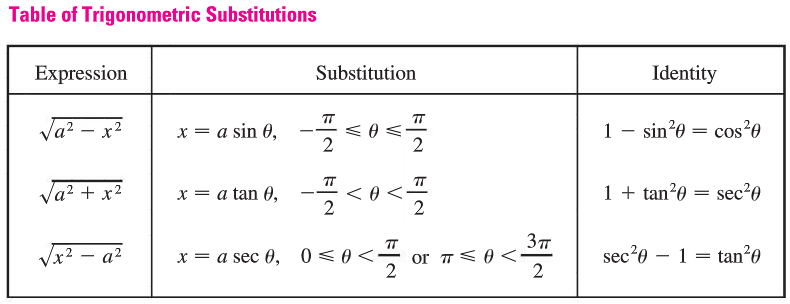
\includegraphics[scale=0.55]{7-3pic1.png}\]
\indent


\underline{Example 1}: Evaluate $\ds\int \ds\frac{\sqrt{9-x^2}}{x^2}dx$.\\
\indent

\vspace{3in}

\underline{Example 2}: Find $\ds\int \ds\frac{1}{x^2\sqrt{x^2 + 4}}dx.$\\
\indent

\vspace{4.5in}

\underline{Example 3}: Find $\ds\int \ds\frac{x}{\sqrt{x^2 + 4}}dx.$\\
\indent

\vspace{4.5in}

\underline{Example 4}: Evaluate $\ds\int \ds\frac{dx}{\sqrt{x^2 - a^2}}, $ where $a>0$.\\
\indent

\vspace{4.5in}
\newpage
\underline{Example 5}: Find $\ds\int_0^{\frac{3\sqrt{3}}{2}} \ds\frac{x^3}{(4x^2 + 9)^{3/2}}dx$.\\
\indent

\vspace{4.5in}

\underline{Example 6}: Evaluate $\ds\int \ds\frac{x}{\sqrt{3-2x-x^2}}dx$.\\
\indent

\vspace{4in}












%----------------------------------------------------------------------------------------

\end{document}